\documentclass[journal,onecolumn]{IEEEtran}
\usepackage{cite}
\usepackage{amsmath,amssymb,amsfonts}
\usepackage{algorithmic}
\usepackage{graphicx}
\usepackage{textcomp}
\usepackage{xcolor}
\usepackage[T1]{fontenc}
\usepackage[spanish,es-noshorthands,es-tabla]{babel}
\renewcommand{\IEEEkeywordsname}{Palabras clave}
\graphicspath{{figuras/}}

\setlength{\parskip}{0.45em}
\makeatletter
\def\subsubsection{\@startsection{subsubsection}{3}{\z@}{1.2ex plus 0.3ex minus
0.2ex}{0.4ex}{\normalfont\normalsize\itshape}}
\makeatother

\begin{document}

\title{Predicción multiclase de riesgo cardiovascular en población adulta}

\author{Enzo Castro, Rodrigo Martínez Jiménez y Pablo Sánchez Mérida
\thanks{Práctica 1 de Machine Learning.
Máster Universitario en Inteligencia Artificial, Universidad de Murcia, curso 2026/2027.}}

\maketitle

\begin{abstract}
\end{abstract}

\begin{IEEEkeywords}
\end{IEEEkeywords}

\section{Introducción}
\subsection{Contexto clínico y motivación}
\IEEEPARstart{L}{as} enfermedades cardiovasculares son una de las principales causas de
mortalidad en el mundo.
Detectar de forma temprana el nivel de riesgo de cada paciente permite adaptar las intervenciones
preventivas y aprovechar mejor los recursos sanitarios.
Con este fin, el Hospital Morales Meseguer ha facilitado los datos de sus pacientes para desarrollar
herramientas predictivas que ayuden a evaluar el riesgo cardiovascular~\cite{enunciado}.

\subsection{Objetivos}
El objetivo es clasificar a los pacientes (adultos) en tres niveles de riesgo cardiovascular (bajo,
moderado y alto) a partir de variables sociodemográficas, clínicas, analíticas y de estilo de vida.
Para ello se analiza la calidad del dataset, se proponen técnicas de preprocesamiento para sus
problemáticas y se comparan varios modelos base y de ensamble con un mismo esquema de validación,
con especial atención a la detección de los pacientes de riesgo alto.

\section{Materiales}

\subsection{Descripción del dataset}
El conjunto de datos incluye 2.254 pacientes y 28 variables~\cite{enunciado}: 27 de entrada y la variable
objetivo, el nivel de riesgo cardiovascular (0: bajo, 1: moderado y 2: alto).
De las variables de entrada, 19 son numéricas: la edad, la presión arterial, el perfil lipídico, la
glucosa y la hemoglobina glicosilada, el índice de masa corporal y el perímetro de cintura,
marcadores analíticos como la proteína C reactiva, el ácido úrico o el aclaramiento de creatinina, y
hábitos como el consumo de alcohol, los años de tabaquismo, el sueño o el ejercicio.
Otras 5 son binarias (tabaquismo activo, hipertensión previa, diabetes, tratamiento con estatinas y
uso de antihipertensivos) y 3 son categóricas: el tipo de alimentación, el nivel de actividad física
y los antecedentes familiares.

\subsection{Análisis exploratorio}

\subsubsection{Variable objetivo y desbalance de clases}
La clase de riesgo bajo agrupa a 1.127 pacientes (50~\%), la de riesgo moderado a 676 (30~\%) y la
de riesgo alto a 451 (20~\%).
El desbalance no es muy grande, pero un modelo que diga siempre riesgo bajo, acertaría la
mitad de los casos sin haber aprendido nada, por lo que la exactitud (\textit{accuracy}) no sirve en este caso para evaluar los
modelos~\cite{tema2}.
Además, la clase minoritaria es la más importante clínicamente: clasificar a un paciente de riesgo
alto como de riesgo bajo lo dejaría sin seguimiento.
Por ello, todas las particiones se hacen de forma estratificada.

\subsubsection{Distribución de las variables}
Las medianas de las variables numéricas cambian de forma ordenada entre las clases, aunque sus
distribuciones se solapan mucho y las clases no son linealmente separables.
Las variables binarias se asocian al riesgo, de la manera esperada: el 56~\% de los pacientes de riesgo
alto tiene hipertensión previa y el 53~\% toma antihipertensivos.
En las categóricas, tiene riesgo alto el 12~\% de los pacientes con dieta mediterránea o
vegetariana, frente al 29~\% de los que siguen la occidental; el riesgo alto baja de forma ordenada
con la actividad física, del 31~\% en los sedentarios al 8~\% en los muy activos; y con los
antecedentes familiares pasa del 12~\% (ninguno) al 22~\% (materno), 28~\% (paterno) y 40~\%
(ambos).

\subsubsection{Valores faltantes}
Cuatro variables tienen valores nulos: el colesterol LDL (6,0~\%), la glucosa en ayunas
(5,0~\%), las horas de sueño (8,0~\%) y la proteína C reactiva (7,0~\%).
Los nulos se reparten entre pacientes distintos, de modo que el 23,6~\% de los pacientes tiene al
menos uno y eliminarlos supondría perder casi uno de cada cuatro.
En cada variable, el porcentaje de nulos apenas cambia entre las tres clases de riesgo (como mucho
2,5 puntos), y al ejecutar un test chi-cuadrado, se confirma que el hecho de que falte un dato no está relacionado
con el riesgo del paciente. Por eso no hace falta añadir indicadores de nulo.

\subsubsection{Calidad de los datos}
La revisión de rangos y de la coherencia entre variables muestra tres tipos de errores de registro,
recogidos en la Tabla~\ref{tab:limpieza}.
El primero son valores imposibles, como consumos de alcohol negativos, un índice de masa corporal
(IMC) de 3,6 o edades de 9,8 y 14,4 años en pacientes que llevan más de 12 años fumando.
El segundo son incoherencias entre variables: en 44 pacientes la presión sistólica es menor o igual
que la diastólica, y en 559 (el 25~\%) la suma de HDL y LDL supera al colesterol total.
El tercero son valores repetidos, de forma sospechosa: en la presión sistólica, el colesterol total, los
triglicéridos y el ácido úrico aparecen dos valores con decimales que se repiten entre 36 y 74 veces
(por ejemplo, 452,7~mg/dL en los triglicéridos), cuando el siguiente valor más frecuente se repite
como mucho 16 veces.
Estos valores están por encima del máximo del resto de pacientes, afectan al 4--6~\% de ellos y esos
pacientes no tienen más riesgo que el resto, por lo que se interpretan como nulos camuflados: 449
valores en total.

\subsubsection{Correlaciones y redundancia}
Se usa la correlación de Spearman en lugar de la de Pearson, porque varias variables tienen
distribuciones asimétricas y el riesgo es una variable con orden (bajo, moderado y alto), no una
medida continua.
Spearman trabaja con el orden de los valores, así que no le afectan ninguna de las dos.
Ningún par de variables de entrada supera en valor absoluto 0,11, así que no hay variables
redundantes que eliminar.
Además, pares que clínicamente deberían estar relacionados, parecen prácticamente independientes
(presión sistólica y diastólica, 0,01; glucosa y hemoglobina glicosilada, 0,05), lo que, junto con
la incoherencia entre HDL, LDL y colesterol total, sugiere que las variables se generaron de forma
independiente.
Respecto al riesgo, las relaciones más importantes son el consumo de alcohol (0,39), la hemoglobina
glicosilada (0,28), la proteína C reactiva (0,28) y el uso de antihipertensivos (0,24), y las
negativas más marcadas, la frecuencia de ejercicio ($-0{,}21$) y el colesterol HDL ($-0{,}20$).
Todas son débiles o moderadas, puesto que el riesgo depende de la combinación de muchas variables y no de una
sola.

\subsection{Problemáticas detectadas}
El análisis exploratorio identifica los siguientes problemas, los cuales se tratan en el preprocesamiento de
la Sección~\ref{sec:metodos}:
\begin{itemize}
\item Valores faltantes en 4 variables, que pasan a 12 tras corregir los errores de registro.
\item Errores de registro: valores imposibles, incoherencias entre variables y nulos camuflados.
\item Desbalance de clases, con la clase de riesgo alto como minoritaria.
\item Variables categóricas en texto, que los modelos no pueden usar directamente.
\item Escalas muy distintas entre variables y presencia de valores extremos.
\end{itemize}

\section{Métodos}\label{sec:metodos}

\subsection{Preprocesamiento}

\subsubsection{Limpieza de errores de registro}
Los errores de registro se corrigen mediante reglas fijas, definidas a partir de los valores
clínicamente posibles de cada variable (Tabla~\ref{tab:limpieza}).
Dado que estas reglas no se estiman a partir de los datos, pueden aplicarse antes de dividir el
conjunto en entrenamiento y test sin riesgo de fuga de datos.
El criterio principal es pasar a nulo los valores imposibles, que después se imputan, salvo cuando el
propio error conserva información sobre el riesgo.
Es el caso del consumo de alcohol en negativo: esos 177 pacientes solo tienen un 2~\% de riesgo alto,
de modo que el valor indica un consumo bajo y se recorta a 0 en lugar de imputarle la mediana (4,3
unidades de bebida a la semana).
De la misma manera, los 41 pacientes con más de 7 días de ejercicio a la semana, con un 5~\% de riesgo
alto, se recortan a 7.
Los cuatro menores de 18 años no se eliminan: al llevar años fumando, son adultos con la edad mal
registrada, así que solo su edad se pasa a nulo y se conservan el resto de datos.
En cuanto al IMC solo se anula lo que es totalmente imposible (menos de 10); entre 10 y 12, estaría dentro de una
desnutrición extrema, pero posible.
La incoherencia entre HDL, LDL y colesterol total no se corrige, porque no se puede saber qué
variable es la errónea y además, afecta a un cuartode los pacientes, por lo que se documenta como limitación del
dataset.

\begin{table}[!t]
\caption{Errores de registro detectados y regla aplicada}
\label{tab:limpieza}
\centering
\begin{tabular}{l c l}
\hline
Problema & Casos & Regla \\
\hline
HDL o triglicéridos negativos & 4 + 4 & Pasar a nulo \\
Consumo de alcohol negativo & 177 & Recortar a 0 \\
IMC menor de 10 & 8 & Pasar a nulo \\
Edad menor de 18 años & 4 & Pasar la edad a nulo \\
Más de 7 días de ejercicio a la semana & 41 & Recortar a 7 \\
Presión sistólica $\leq$ diastólica & 44 & Pasar las dos a nulo \\
Valores repetidos (nulos camuflados) & 449 & Pasar a nulo \\
HDL + LDL $>$ colesterol total & 559 & No se corrige (limitación) \\
\hline
\end{tabular}
\end{table}

\subsubsection{Codificación de variables categóricas}
Las tres variables categóricas se transforman en números con una correspondencia fija entre cada
categoría y su valor.
El nivel de actividad tiene un orden natural, de sedentario a muy activo, y cuanto más activo es el
paciente, menor es el porcentaje de riesgo alto: del 31~\% en los sedentarios baja al 8~\% en los
muy activos.
Por eso se codifica como variable ordinal de 0 a 3, conservando ese orden.
El tipo de alimentación no tiene orden y se codifica con \textit{one-hot}.
Con las cuatro columnas, una siempre se puede deducir de las otras tres, lo que se conoce como
colinealidad perfecta y perjudica a modelos como la regresión logística.
Por eso se elimina la columna de la dieta mediterránea, la de menor riesgo alto (12~\%), que queda
como categoría de referencia: un paciente con las otras tres columnas a 0 sigue la dieta
mediterránea.
Los antecedentes familiares se representan con dos variables binarias, una para la madre y otra para
el padre, de modo que un paciente con antecedentes por ambas partes tiene las dos a 1.
Esta codificación refleja bien cómo influyen en el riesgo: el riesgo alto pasa del 12~\% sin
antecedentes al 22~\% con antecedentes maternos y al 28~\% con paternos, y llega al 40~\% con
ambos, casi la suma de los dos efectos por separado.

\subsubsection{Imputación de valores faltantes}
Tras la limpieza, 12 variables tienen nulos y el 39~\% de los pacientes tiene al menos uno, así que
eliminar filas supondría perder 884 pacientes.
Siguiendo el tratamiento de valores faltantes de la asignatura~\cite{tema1}, para elegir el método
de imputación se realizó un experimento: sobre los 1.370 pacientes sin nulos se ocultaron al azar
valores en la misma proporción que los nulos reales, se reconstruyeron con la media, la mediana, KNN
(5 y 25 vecinos) e \texttt{IterativeImputer}, y se midió el error absoluto medio en 30 repeticiones.
La mediana iguala o mejora a todas las alternativas: KNN con 5 vecinos tiene el mayor error en las
12 variables, y la mayor ventaja de \texttt{IterativeImputer} (0,2~mg/dL en la glucosa) queda muy
por debajo de la variación entre repeticiones.
Tiene sentido, porque las variables con nulos apenas se relacionan con el resto (la correlación más
alta es de 0,12): KNN e \texttt{IterativeImputer} estiman el valor que falta a partir de las demás
variables del paciente, y si estas no aportan información sobre él, no pueden hacerlo mejor que la
mediana.
Por el mismo motivo se descartó calcular el LDL con la fórmula de Friedewald, cuyo error
(47,4~mg/dL) supera al de la mediana (29,5~mg/dL).
La imputación con la mediana se realiza dentro del \textit{pipeline}, de modo que la mediana se
calcula solo con los datos de entrenamiento de cada fold.

\subsubsection{Escalado}
Las variables numéricas se escalan con \texttt{RobustScaler}, que usa la mediana y el rango
intercuartílico y es menos sensible a los valores extremos que la estandarización.
Se aplica en todos los modelos: a los basados en árboles no les afecta, porque el escalado no cambia
el orden de los valores, pero SMOTENC busca vecinos por distancia y, sin escalar, la dominarían el
colesterol y los triglicéridos.
Las variables binarias y categóricas no se escalan.

\subsubsection{Tratamiento del desbalance}
Se comparan varias opciones en cada modelo: no balancear; \texttt{class\_weight} con la opción
\texttt{balanced}, que aplica el aprendizaje sensible al coste~\cite{tema2} y pondera el error de
cada clase de forma inversa a su frecuencia (pesos de 0,67, 1,11 y 1,66 para riesgo bajo, moderado y
alto); SMOTENC~\cite{tema2,nb_desbalanceo}, que genera pacientes sintéticos de las clases
minoritarias hasta igualarlas (901 por clase en el entrenamiento); y
Tomek~\cite{nb_desbalanceo}, que elimina pacientes de las clases mayoritarias situados en la
frontera con otra clase.
Se utiliza SMOTENC y no SMOTE porque SMOTE interpola también las variables binarias y categóricas: con
el mismo preprocesado, 2.967 de los 9.900 valores categóricos de sus pacientes sintéticos tenían
decimales (por ejemplo, un fumador con valor 0,67), frente a ninguno con SMOTENC, que asigna la
categoría más frecuente entre los vecinos.
Las técnicas de remuestreo se aplican dentro del \textit{pipeline} de \texttt{imbalanced-learn},
solo sobre los datos de entrenamiento de cada fold, de modo que la validación se hace siempre con
pacientes reales.

\subsubsection{Técnicas descartadas}
Además de las ya mencionadas (Friedewald, KNN e \texttt{IterativeImputer} para imputar, y SMOTE para
balancear), se descartaron también:
\begin{itemize}
\item Eliminar los pacientes con nulos, porque se perdería el 39~\% de la muestra.
\item Pasar a nulo los valores fuera de unos rangos clínicos de referencia.
Una vez quitados los nulos camuflados, solo 134 valores se salen de ellos y no parecen errores: en
el HDL, la proteína C reactiva y la hemoglobina glicosilada, entre el 29 y el 30~\% de esos
pacientes es de riesgo alto, frente al 20~\% del total.
\item Eliminar variables por correlación, porque ningún par supera el valor de 0,11.
\end{itemize}

\subsection{Esquema de validación}
Los datos se dividen una sola vez en entrenamiento (80~\%, 1.803 pacientes) y test (20~\%, 451
pacientes), de forma estratificada para mantener la proporción de clases en ambos conjuntos.
El test se reserva para una única evaluación final.
Los modelos se ajustan y comparan con validación cruzada estratificada de 5
folds~\cite{tema1,nb_metricas} (\texttt{StratifiedKFold} con mezcla aleatoria), con la misma semilla (42) y
los mismos folds para todos, lo que permite comparar los modelos fold a fold.
Todo lo que se aprende de los datos forma parte de un \textit{pipeline} común, construido con
scikit-learn e \texttt{imbalanced-learn}: imputación y escalado de las variables numéricas, balanceo
y modelo.
Se ajusta solo con los folds de entrenamiento, lo que evita la fuga de información a validación.
La partición, los folds de validación, las métricas y el \textit{pipeline} se definen en un único módulo
utilizado por todo el grupo.

\subsection{Métricas de evaluación}
Se utilizan F1, precisión y recall, en su versión macro, que da el mismo peso a las tres clases y
evita que domine la mayoritaria~\cite{tema1,tema2}.
La métrica más crítica es el recall de la clase de riesgo alto: un falso negativo deja a un paciente
de riesgo alto sin seguimiento ni tratamiento preventivo, mientras que un falso positivo supone
pruebas o tratamientos innecesarios, provocando un coste menor.
Aun así, el recall no se usa para elegir hiperparámetros, porque un modelo que clasificara a todos
los pacientes como de riesgo alto tendría un recall de 1 y sería inútil (su F1 macro sería de 0,11).
Por eso los modelos se ajustan con el F1 macro, que equilibra precisión y recall en las tres clases.
El recall de riesgo alto se utiliza después de dos formas: para elegir entre modelos con un F1 macro
parecido y para analizar sus errores desde el punto de vista clínico.
En ese análisis, se utiliza también la precisión de esa clase, que indica cuántas de las alarmas del
modelo son correctas y la matriz de confusión, que muestra si un paciente de riesgo alto se
clasifica como riesgo moderado o como bajo.

\subsection{Modelos}

\subsubsection{Modelos base}

\textit{Árbol de decisión.} Clasifica a los pacientes mediante una secuencia de preguntas sobre
sus variables, por ejemplo si la proteína C reactiva supera un cierto umbral.
En cada paso elige la variable y el umbral que mejor separan las clases, es decir, los que dejan
grupos de pacientes lo más homogéneos posible.
Sus decisiones se pueden leer directamente, pero si crece sin límite acaba memorizando los datos de
entrenamiento.
Se ajustan la medida de homogeneidad (Gini o entropía), la profundidad máxima (3, 5, 8, 12 o sin
límite) y el número mínimo de pacientes por hoja (1, 5 o 20), que controlan cuánto puede crecer.

\textit{k vecinos más cercanos (kNN).} Asigna a cada paciente la clase más frecuente entre los $k$
pacientes del entrenamiento más parecidos a él.
Como el parecido se mide con distancias, necesita que las variables estén escaladas, si no, las de
valores más grandes dominarían el cálculo.
Se ajustan el número de vecinos (de 3 a 75) y la forma de medir la distancia (euclídea o
Manhattan).
No admite \texttt{class\_weight}, porque no aprende parámetros a los que se pueda dar peso: solo
compara cada paciente con los del entrenamiento.

\subsubsection{Modelos de ensamble}

\textit{Random Forest.} Es un ensamble de tipo \textit{bagging}~\cite{tema2,nb_ensambles}: combina
numerosos árboles de decisión y clasifica a cada paciente mediante votación entre ellos.
Para que los árboles sean distintos entre sí, cada uno se entrena con una muestra aleatoria de los
pacientes, tomada con reemplazo (\textit{bootstrap}), y en cada división solo puede elegir entre un
subconjunto aleatorio de variables.
Así, aunque cada árbol por separado sobreajuste, sus errores se compensan al promediarlos y el
conjunto generaliza mejor que un único árbol.
Se ajustan el número de árboles (100 o 300), la profundidad máxima (5, 10 o sin límite), el número
de variables que se prueban en cada división (la raíz cuadrada del total o la mitad) y el número
mínimo de pacientes por hoja (1, 5 o 10).

\subsection{Ajuste de hiperparámetros}
Todos los modelos se ajustan con búsqueda en rejilla (\texttt{GridSearchCV})~\cite{nb_metricas}
sobre la validación cruzada.
En cada combinación se calculan todas las métricas, en entrenamiento y en validación, y se elige la
de mayor F1 macro.
Con el mismo criterio se elige la técnica de balanceo de cada modelo: el F1 macro y, si la
diferencia queda dentro de la desviación entre folds, se escoge por el recall de riesgo alto.

\subsection{Comparación estadística de modelos}

\subsection{Entorno y reproducibilidad}
El código está en el repositorio de GitHub (\texttt{github.com/enzocastrozn/machine\_learning}), con
Python 3.12 y las versiones de las dependencias fijadas con uv y en \texttt{requirements.txt}.
Se usa una única semilla (42) en la partición, los folds, el remuestreo y los modelos.
Los notebooks de cada miembro comparten el módulo de preprocesamiento y validación, y guardan los
resultados de validación, incluida la nota de cada fold, para la comparación final.

\section{Análisis de resultados}

\subsection{Comparación de técnicas de preprocesamiento}
La Tabla~\ref{tab:preprocesamiento} muestra el F1 macro y el recall de riesgo alto en validación de
cada modelo con cada técnica de balanceo.
En el árbol de decisión las cuatro opciones empatan en F1 macro (entre 0,532 y 0,545, dentro de la
desviación entre folds), pero balancear con \texttt{class\_weight} o con SMOTENC eleva el recall de
riesgo alto de 0,50 a 0,60; se elige SMOTENC por su mayor precisión en esa clase.
En kNN, SMOTENC mejora ambas métricas (F1 de 0,537 a 0,590 y recall de 0,41 a 0,77).
En Random Forest, \texttt{class\_weight} obtiene el mejor F1 macro (0,648) y el mejor recall de
riesgo alto (0,72).
Tomek no es la mejor opción en ningún modelo: solo elimina 182 pacientes de la frontera (82 de
riesgo bajo y 100 moderados) y ninguno de riesgo alto, así que el desbalance se mantiene (819, 441 y
361 pacientes).
Se concluye que no hay una técnica de balanceo mejor para todos los modelos, lo que justifica haberlas
comparado en cada uno en lugar de fijar una sola técnica para todos.

\begin{table}[!t]
\caption{F1 macro y, entre paréntesis, recall de riesgo alto en validación según la técnica de
balanceo.
En negrita, la técnica elegida en cada modelo}
\label{tab:preprocesamiento}
\centering
\begin{tabular}{l c c c c}
\hline
Modelo & Sin balancear & \texttt{class\_weight} & SMOTENC & Tomek \\
\hline
Árbol de decisión & 0,545 (0,50) & 0,532 (0,60) & \textbf{0,541 (0,60)} & 0,540 (0,52) \\
kNN & 0,537 (0,41) & -- & \textbf{0,590 (0,77)} & 0,549 (0,49) \\
Random Forest & 0,611 (0,56) & \textbf{0,648 (0,72)} & 0,627 (0,69) & 0,609 (0,68) \\
\hline
\end{tabular}
\end{table}

\subsection{Resultados en validación cruzada}
La Tabla~\ref{tab:resultados} resume la mejor configuración de cada modelo.
Entre el árbol de decisión, kNN y Random Forest, el mejor F1 macro corresponde a Random Forest, que
supera a kNN en los cinco folds (por 0,058, 0,065, 0,057, 0,088 y 0,025). kNN, en cambio, obtiene el
mayor recall de riesgo alto y solo clasifica como riesgo bajo a 8 de los 361 pacientes de riesgo
alto del entrenamiento, a costa de más falsas alarmas: su precisión de riesgo alto es de 0,56,
frente a 0,65 en Random Forest.

\begin{table}[!t]
\caption{Mejor configuración de cada modelo en validación cruzada (media $\pm$ desviación entre
folds)}
\label{tab:resultados}
\centering
\begin{tabular}{l l c c c c}
\hline
Modelo & Balanceo & F1 macro & Recall alto & Precisión alto & Alto $\rightarrow$ bajo \\
\hline
Árbol de decisión & SMOTENC & 0,541 $\pm$ 0,033 & 0,60 & 0,50 & 37 \\
kNN & SMOTENC & 0,590 $\pm$ 0,020 & 0,77 & 0,56 & 8 \\
Random Forest & \texttt{class\_weight} & 0,648 $\pm$ 0,035 & 0,72 & 0,65 & 10 \\
\hline
\end{tabular}
\end{table}

\subsection{Análisis del sobreajuste}
La Fig.~\ref{fig:curvas} muestra las curvas de validación del árbol de decisión y de kNN.
En el árbol, a partir de profundidad 4, la validación oscila entre 0,51 y 0,54 mientras el
entrenamiento sube hasta 0,87: por lo que la profundidad adicional solo sirve para memorizar pacientes.
La mejor combinación (entropía, sin límite de profundidad y 5 pacientes por hoja; 0,867 en
entrenamiento frente a 0,541 en validación) empata con otra mucho más sencilla (Gini, profundidad 12
y 20 pacientes por hoja), que obtiene 0,540~$\pm$~0,008 con solo 0,693 en entrenamiento y sería
preferible por su menor sobreajuste.
En kNN se aprecia el compromiso entre sesgo y varianza: con un vecino el entrenamiento es perfecto y
la validación se queda en 0,50; al aumentar el número de vecinos, la validación sube hasta estabilizarse
entre 31 y 51, y el valor elegido (51) apenas sobreajusta (0,635 frente a 0,590).
Random Forest alcanza 0,997 en entrenamiento, pero es el que mejor generaliza, con 0,107 más en
validación que el árbol individual: cada árbol sobreajusta por separado, pero al promediar muchos
árboles distintos se reduce la varianza, además, limitar a 10 los pacientes por hoja reduce su F1 de entrenamiento a 0,90 sin empeorar la validación.

\begin{figure}[!t]
\centering
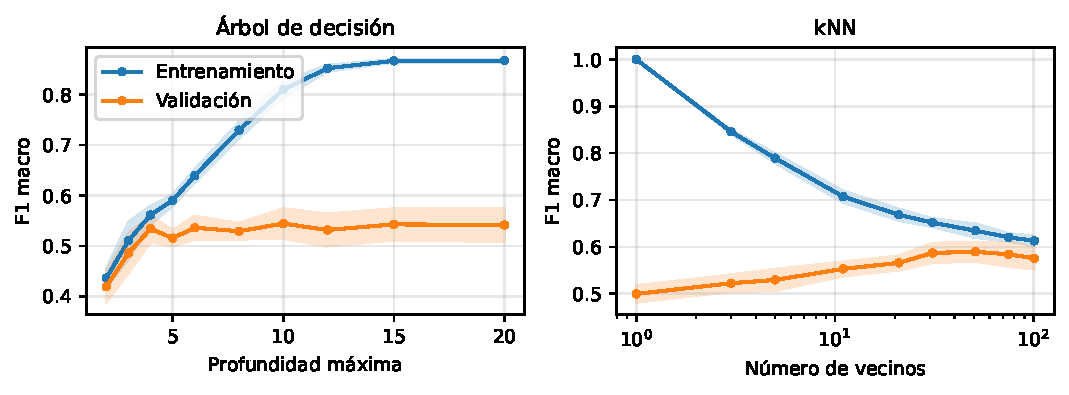
\includegraphics[width=0.85\linewidth]{curvas_validacion.pdf}
\caption{Curvas de validación del árbol de decisión (profundidad máxima) y de kNN (número de
vecinos): F1 macro en entrenamiento y validación, con la media y la desviación entre folds.}
\label{fig:curvas}
\end{figure}

\subsection{Matrices de confusión y errores clínicamente graves}

\subsection{Importancia de las variables}
La importancia por permutación~\cite{tema2,nb_ensambles} de Random Forest se calcula en los folds de
validación, porque en entrenamiento el modelo memoriza a los pacientes y las variables se compensan
entre sí.
Las más relevantes son la proteína C reactiva y el consumo de alcohol, seguidas a distancia por el
ácido úrico y la hemoglobina glicosilada (Fig.~\ref{fig:importancia}), concordando con las
correlaciones del análisis exploratorio.
Otras variables relacionadas con el riesgo en ese análisis, como el HDL o la frecuencia de
ejercicio, tienen una importancia dentro del ruido entre folds: no significa que no estén
relacionadas con el riesgo, sino que el modelo apenas pierde F1 al desordenarlas, probablemente
porque su efecto es pequeño frente al de las dos primeras.
El árbol de decisión confirma esta jerarquía y permite leer sus umbrales en unidades clínicas
deshaciendo el escalado: su primer corte separa a los pacientes con una proteína C reactiva de
0,97~mg/L, muy próximo al umbral de 1~mg/L que la AHA y los CDC emplean para el riesgo
cardiovascular bajo.

\begin{figure}[!t]
\centering
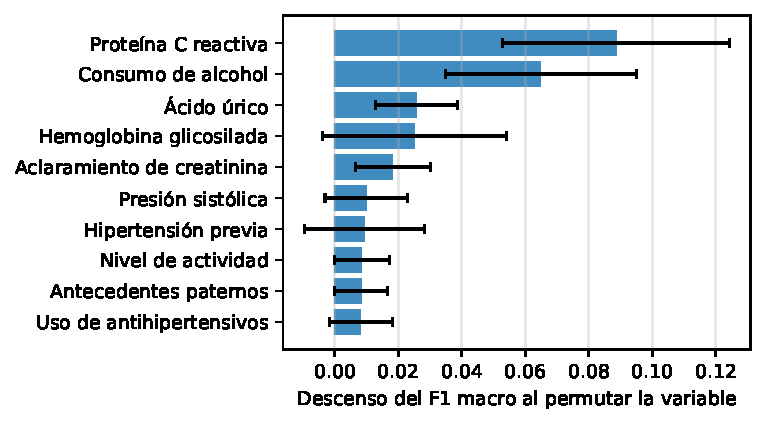
\includegraphics[width=0.62\linewidth]{importancia_rf.pdf}
\caption{Importancia por permutación de las 10 variables más relevantes para Random Forest: descenso
medio del F1 macro en los folds de validación y su desviación.}
\label{fig:importancia}
\end{figure}

\subsection{Test estadísticos}

\subsection{Evaluación final en test}

\section{Discusión y conclusiones}

\subsection{Mejor modelo y justificación}

\subsection{Complejidad, interpretabilidad y robustez}

\subsection{Limitaciones del dataset}

\subsection{Posibles mejoras y trabajo futuro}

\bibliographystyle{IEEEtran}
\bibliography{referencias}

\end{document}
